\section{Experiments}

\subsection{setup}
\paragraph{Evaluation Datasets}

We comprehensively evaluated our method using 3 text-based protein understanding datasets: \blackcircle{1} ProtDescribe~\cite{xu2023protst} comprises 553,052 high-quality protein–text pairs extracted from Swiss-Prot. Each instance pairs an amino-acid sequence with a single textual description obtained by concatenating four annotation fields in a fixed order: protein name, function, subcellular location, and similarity. The resulting descriptions average 40–60 tokens.
% 
\blackcircle{2} Protein2Text-QA~\cite{Protein2Text2025} comprises 209,847 open-ended question–answer pairs covering 5,574 unique proteins. Each instance consists of an amino-acid sequence, a free-form question, and a concise answer; all QAs are automatically generated from PubMed abstracts/discussion/introduction sections and presented as conversational natural-language text without fixed templates.
% 
\blackcircle{3} Mol-Instructions~\cite{fang2023mol} comprises 2.04 M instruction instances divided into three major sections: molecule-oriented, protein-oriented, and biomolecular-text. The protein-oriented section alone contributes 505 K instructions covering diverse tasks. Each sample is formatted as a natural-language “instruction–input–output” triplet: the input is a UniProt amino-acid sequence, and the output is a free-text answer tailored to the specific task.


\paragraph{Models} All experiments are conducted under identical prompting protocols. We first evaluate the proposed adaptive context construction method on frozen LLMs, including Qwen2.5-3B~\cite{qwen2.5}, Mistral-7B-Instruct-v0.3~\cite{chaplot2023albert}, Qwen3-14B~\cite{qwen3technicalreport}, Kimi-k2~\cite{team2025kimi}, and GPT-4o~\cite{openai2024gpt4}, to test few-shot and compositional reasoning capabilities, thereby mimicking the dynamics of second language acquisition. In addition, we also evaluate fine-tuned protein-oriented LLMs, such as BioT5-plus-base~\cite{pei2023biot5} and ProLLaMA~\cite{lv2025prollama}, which have been explicitly trained on large-scale protein corpora. These models serve as a baseline for comparison, allowing us to examine the performance gains of our method in general-purpose frozen LLMs relative to specialized protein LLMs.


\paragraph{Metrics} 

We evaluate model outputs using both an automatic metric (ROUGE-L~\cite{lin2002manual}) and human evaluation. ROUGE-L~\cite{lin2002manual}, though widely used for text generation, primarily measures lexical overlap and may not fully capture semantic correctness in protein-related QA. To address this limitation, five evaluators rated the quality of generated answers on a 0–5 scale, where 0 denotes garbled and unreadable content, intermediate scores reflect increasing levels of informativeness and accuracy, and 5 represents fully correct outputs (detailed scoring rubrics are provided in Appendix~\ref{appendix:human_rate}). This combined evaluation provides a more reliable assessment of factual accuracy and overall comprehensibility.


\subsection{Quality of Dataset}
Figure~\ref{fig:dataset} (a-f) provides a multidimensional analysis of the protein sequences included in our dataset. The collection spans a wide range of sequence lengths, from short peptides to large multi-domain proteins, and covers proteins from 4,135 species across diverse evolutionary lineages. At the family level, the dataset comprises 63,749 families and 1,115 superfamilies, ensuring representation of both well-studied proteins and rare functional groups. Additional annotations capture domain composition, catalytic activity classes, and gene ontology categories, collectively highlighting the long-tail distribution across sequence space and functional categories. 
% 
This diversity ensures broad biological coverage while posing realistic challenges in inferring functions for proteins, particularly for infrequent families and underexplored functions.

Figure~\ref{fig:dataset} (g,h) summarizes the distribution of tasks and token composition within the dataset. The corpus encompasses four distinct protein-QA types, with sample counts ranging from 11,693 (attribute-based QA) to 32,444 (true/false QA), thereby providing balanced coverage across multiple functional perspectives. 
% 
In terms of token composition, amino-acid sequences constitute nearly 70 \% of the corpus, reflecting the sequence-centric nature of protein understanding tasks and highlighting the need for models to align symbolic sequence information with natural-language context effectively.

\begin{figure}[ht]
\centering
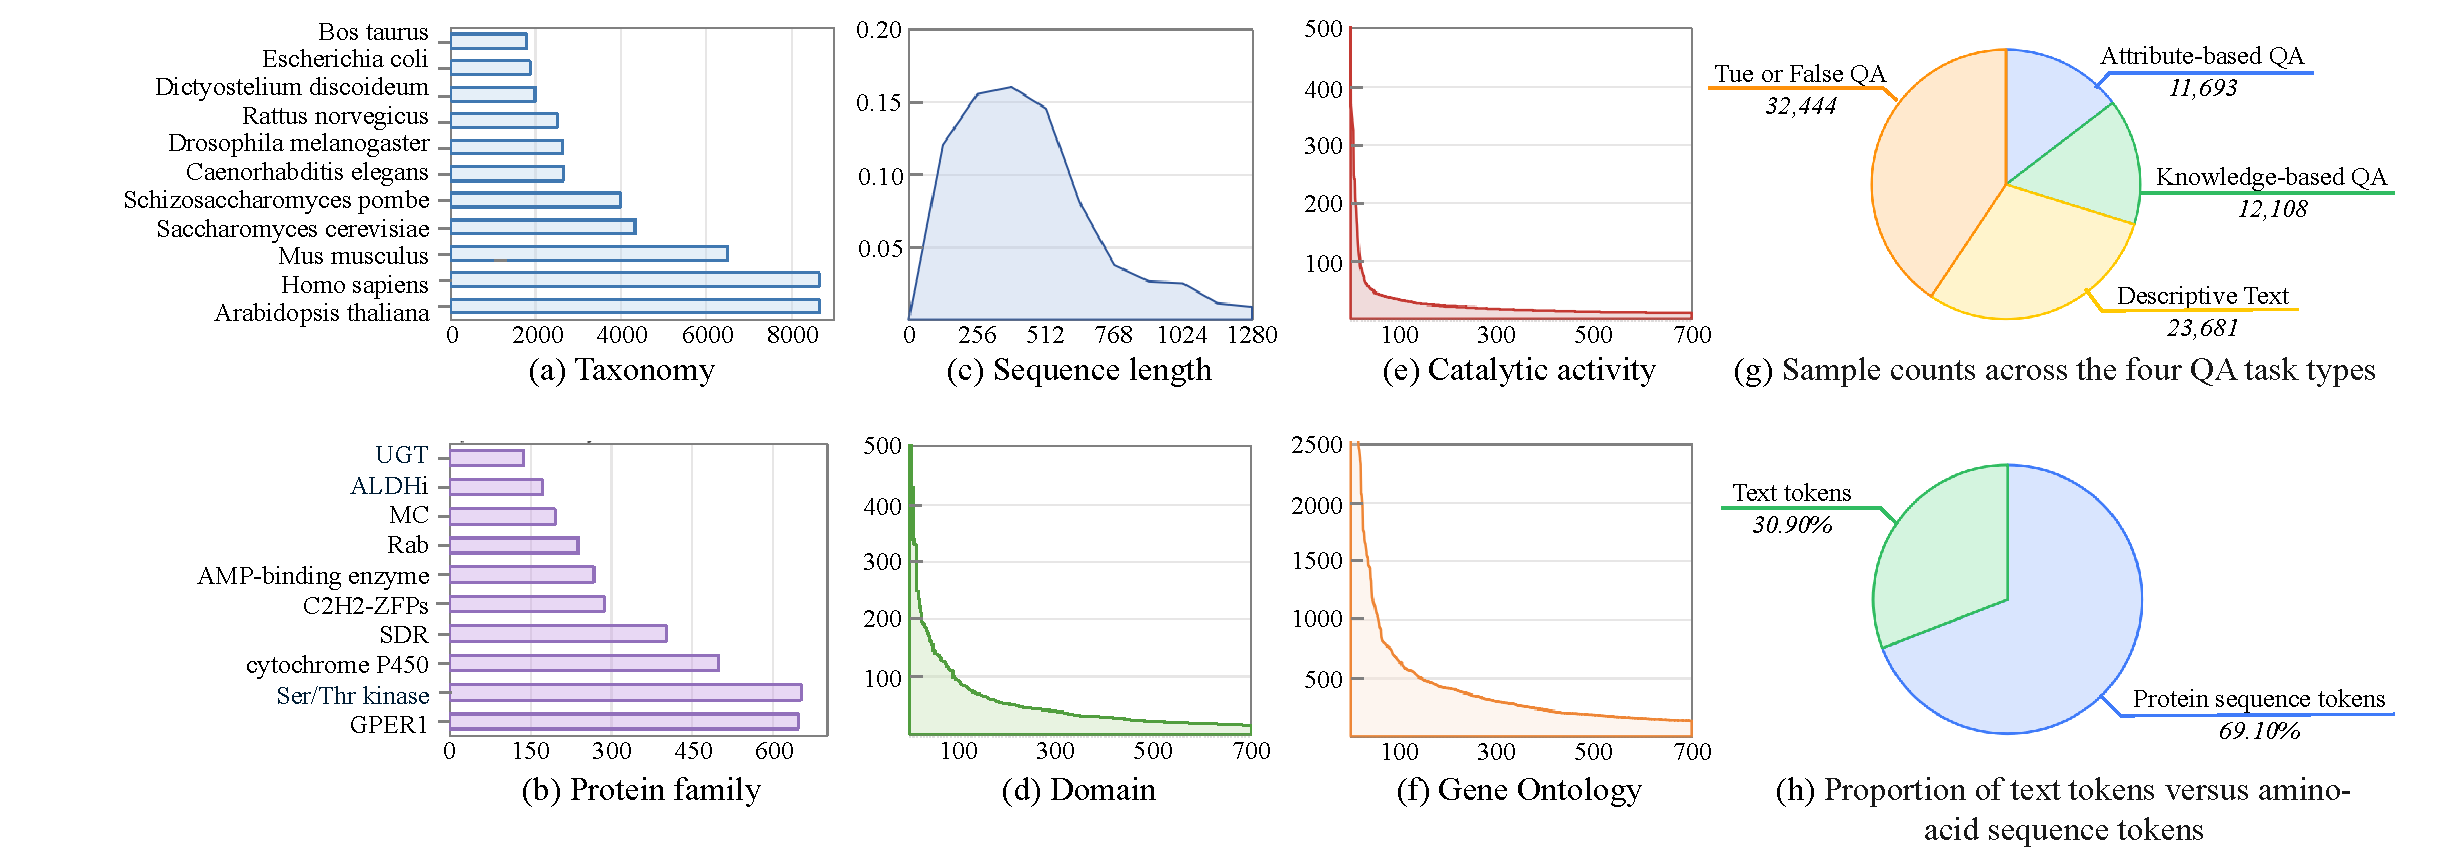
\includegraphics[width=\linewidth]{figure/dataset_analysis_0.pdf}
\caption{\textbf{Dataset statistics.} 
Left: Multidimensional analysis of protein amino-acid sequences, including length, domain composition, and catalytic activity. Right: Sample sizes for the four protein-QA types and the ratio of textual to amino-acid sequence tokens.
}
\label{fig:dataset}
\end{figure}

\subsection{Main Results}
\paragraph{Accuracy gains from context-driven exposure}

Table~\ref{tab:main} presents that our method consistently improves performance on three text-based protein understanding datasets.
% 
Our method raises the average ROUGE-L by 7\% across diverse open-source models and GPT-4o~\cite{openai2024gpt4}, with a maximum gain of 17.2\%, demonstrating that context-driven exposure allows LLMs to acquire protein semantics and reason about function directly from sequence and textual context without any parameter updates. 
% 
Larger models benefit more, suggesting that greater capacity enhances the ability to leverage contextual cues, consistent with learning protein meaning through in-context analogy and reasoning.
% 
In contrast, fine-tuned protein LLMs such as ProLLaMA-7B~\cite{lv2025prollama} do not surpass frozen LLMs augmented with our method, likely due to limited training coverage and task-specific rigidity. This underscores the our method as a lightweight alternative that enables general-purpose LLMs to potentially exceed the performance of domain-adapted models.

\begin{table}[t]
\small
\centering
\setlength{\tabcolsep}{4pt}
\renewcommand\arraystretch{1.2}
    \centering\small
      \caption{\textbf{
  Comparison of different approaches in protein question answering
  } ``Fun.'', ``Des.'', ``Dom.'', and ``Cat.'' denote the 4 protein-oriented tasks in the Mol-Instructions dataset~\cite{fang2023mol}: protein function prediction (Fun.), general textual description generation (Des.), domain/motif recognition (Dom.), and catalytic activity prediction (Cat.). $\Delta$ \textit{Gain} shows the percentage performance increase. $\diamondsuit$ indicates LLMs augmented with our adaptive context construction method. Metric: ROUGE-L.
  }
  \vspace{\baselineskip}
    \begin{tabular}{l|c|c|c@{\hspace{8pt}}c@{\hspace{8pt}}c@{\hspace{8pt}}c@{\hspace{8pt}}c}
\hline

\hline

\hline

\hline
        \multirow{2}{*}{\bf Model}& \multirow{2}{*}{\bf ProtDescribe
} &  \multicolumn{1}{c|}{ \bf Protein2Text-
}&\multicolumn{5}{c}{\bf Mol-Instructions}  \\
          & & \bf QA & Func. & Desc.
 & Dom. & Cat. & \bf Avg.  \\ 
\hline
\rowcolor{gray!20}
        \textit{Fine-tuned LLM} &&&&&&&\\
        BioT5+~\cite{pei2023biot5} & 9.97 & 6.96 & 2.92 & 6.22 & 2.37 & 2.87 & 3.60 \\
        ProLLaMA-7B~\cite{lv2025prollama}& 12.77 & 10.09 & 16.89 & 15.34 & 15.85 & 19.32 & 16.85 \\
\hline
\rowcolor{gray!20} 
        \textit{Frozen LLM} &&&&&&&\\
        Qwen2.5-3B~\cite{qwen2.5} & 18.45 & 23.21 & 18.91 & 17.18 & 18.01 & 20.05 & 18.54 \\
        \rowcolor[HTML]{E6F7FF}
        Qwen2.5-3B~\cite{qwen2.5} $\diamondsuit$& 27.32 & 28.66 & 22.05 & 22.23 & 25.14 & 15.96 & 21.35\\
        $\Delta$ \it Gain & \bf {\color[HTML]{006400} +8.87} & \bf {\color[HTML]{006400} +5.45} & & & & & \bf {\color[HTML]{006400} +2.81}\\
        Mistral-7B-Instruct-v0.3~\cite{chaplot2023albert} & 15.02 & 20.97 & 17.05 & 18.59 & 14.95 & 18.07 & 17.17\\
        \rowcolor[HTML]{E6F7FF}
        Mistral-7B-Instruct-v0.3~\cite{chaplot2023albert} $\diamondsuit$ & 29.39 & 28.59 & 15.77 &22.72 & 17.46 & 21.20 & 19.29\\
        $\Delta$ \it Gain & \bf {\color[HTML]{006400} +14.37} & \bf {\color[HTML]{006400} +7.62} & & & & & \bf {\color[HTML]{006400} +2.12}\\
        Qwen3-14B~\cite{qwen3technicalreport} &  23.20 & 21.02 & 15.80  &  12.75 & 15.81 & 14.06 & 14.61 \\
        \rowcolor[HTML]{E6F7FF}
        Qwen3-14B~\cite{qwen3technicalreport} $\diamondsuit$ &  35.53 & 25.93 & 20.17 & 17.37 & 18.47 & 23.25 & 19.82\\
        $\Delta$ \it Gain & \bf {\color[HTML]{006400}+12.33} & \bf {\color[HTML]{006400} +4.91 } & & & & & \bf {\color[HTML]{006400} +5.21}\\
        % Llama-3.3-70B-Instruct\\
        % \rowcolor[HTML]{E6F7FF}
        % Llama-3.3-70B-Instruct $\diamondsuit$\\
        % $\Delta$ \it Gain & \bf {\color[HTML]{006400}+} & \bf {\color[HTML]{006400} + } & & & & & \bf {\color[HTML]{006400} +}\\
        kimi-k2~\cite{team2025kimi} & 26.74 & 17.33 & 12.60 &12.36 & 10.32 & 15.97 & 12.81 \\
        \rowcolor[HTML]{E6F7FF}
        kimi-k2~\cite{team2025kimi} $\diamondsuit$ & 35.91 & 21.04 & 14.47 & 14.97 & 15.68 & 17.02 & 15.54\\
        $\Delta$ \it Gain & \bf {\color[HTML]{006400} +9.17} & \bf {\color[HTML]{006400} +3.71} & & & & & \bf {\color[HTML]{006400} +2.72}\\
        GPT-4o~\cite{openai2024gpt4} & 18.29 &20.84 & 16.89 & 14.50 & 16.74 & 20.00 & 17.03\\
        \rowcolor[HTML]{E6F7FF}
        GPT-4o~\cite{openai2024gpt4} $\diamondsuit$ &35.53 & 26.86 & 20.24 & 19.23 & 17.46 & 22.61 & 19.89\\
        $\Delta$ \it Gain & \bf {\color[HTML]{006400} +17.22} & \bf {\color[HTML]{006400} +6.02} & & & & & \bf {\color[HTML]{006400} +2.85}\\
        \cline{1-4}
\hline

\hline

\hline

\hline
    \end{tabular}
    
    \label{tab:main}
\end{table}

Human evaluation further demonstrates that exposing models to curated protein–language contexts improves the perceived quality of outputs (Figure~\ref{fig:human_rating}).
% 
Across all rated instances, inter-rater consistency was substantial (Krippendorff’s $\alpha$ = 0.72\%), ensuring reliable annotations; the detailed rubric is given in Appendix~\ref{appendix:human_rate}.
% 
Models receiving context-driven exposures achieve higher or comparable ratings on most tasks (left panel), with the clearest improvements observed on Protein2Text-QA~\cite{Protein2Text2025} and several Mol-Instructions~\cite{fang2023mol} subtasks.
% 
Furthermore, pairwise win/lose analyses (right panel) show that outputs generated with context-driven exposure are preferred in the majority of comparisons, with win rates systematically exceeding loss rates.
\begin{figure}[ht]
\centering
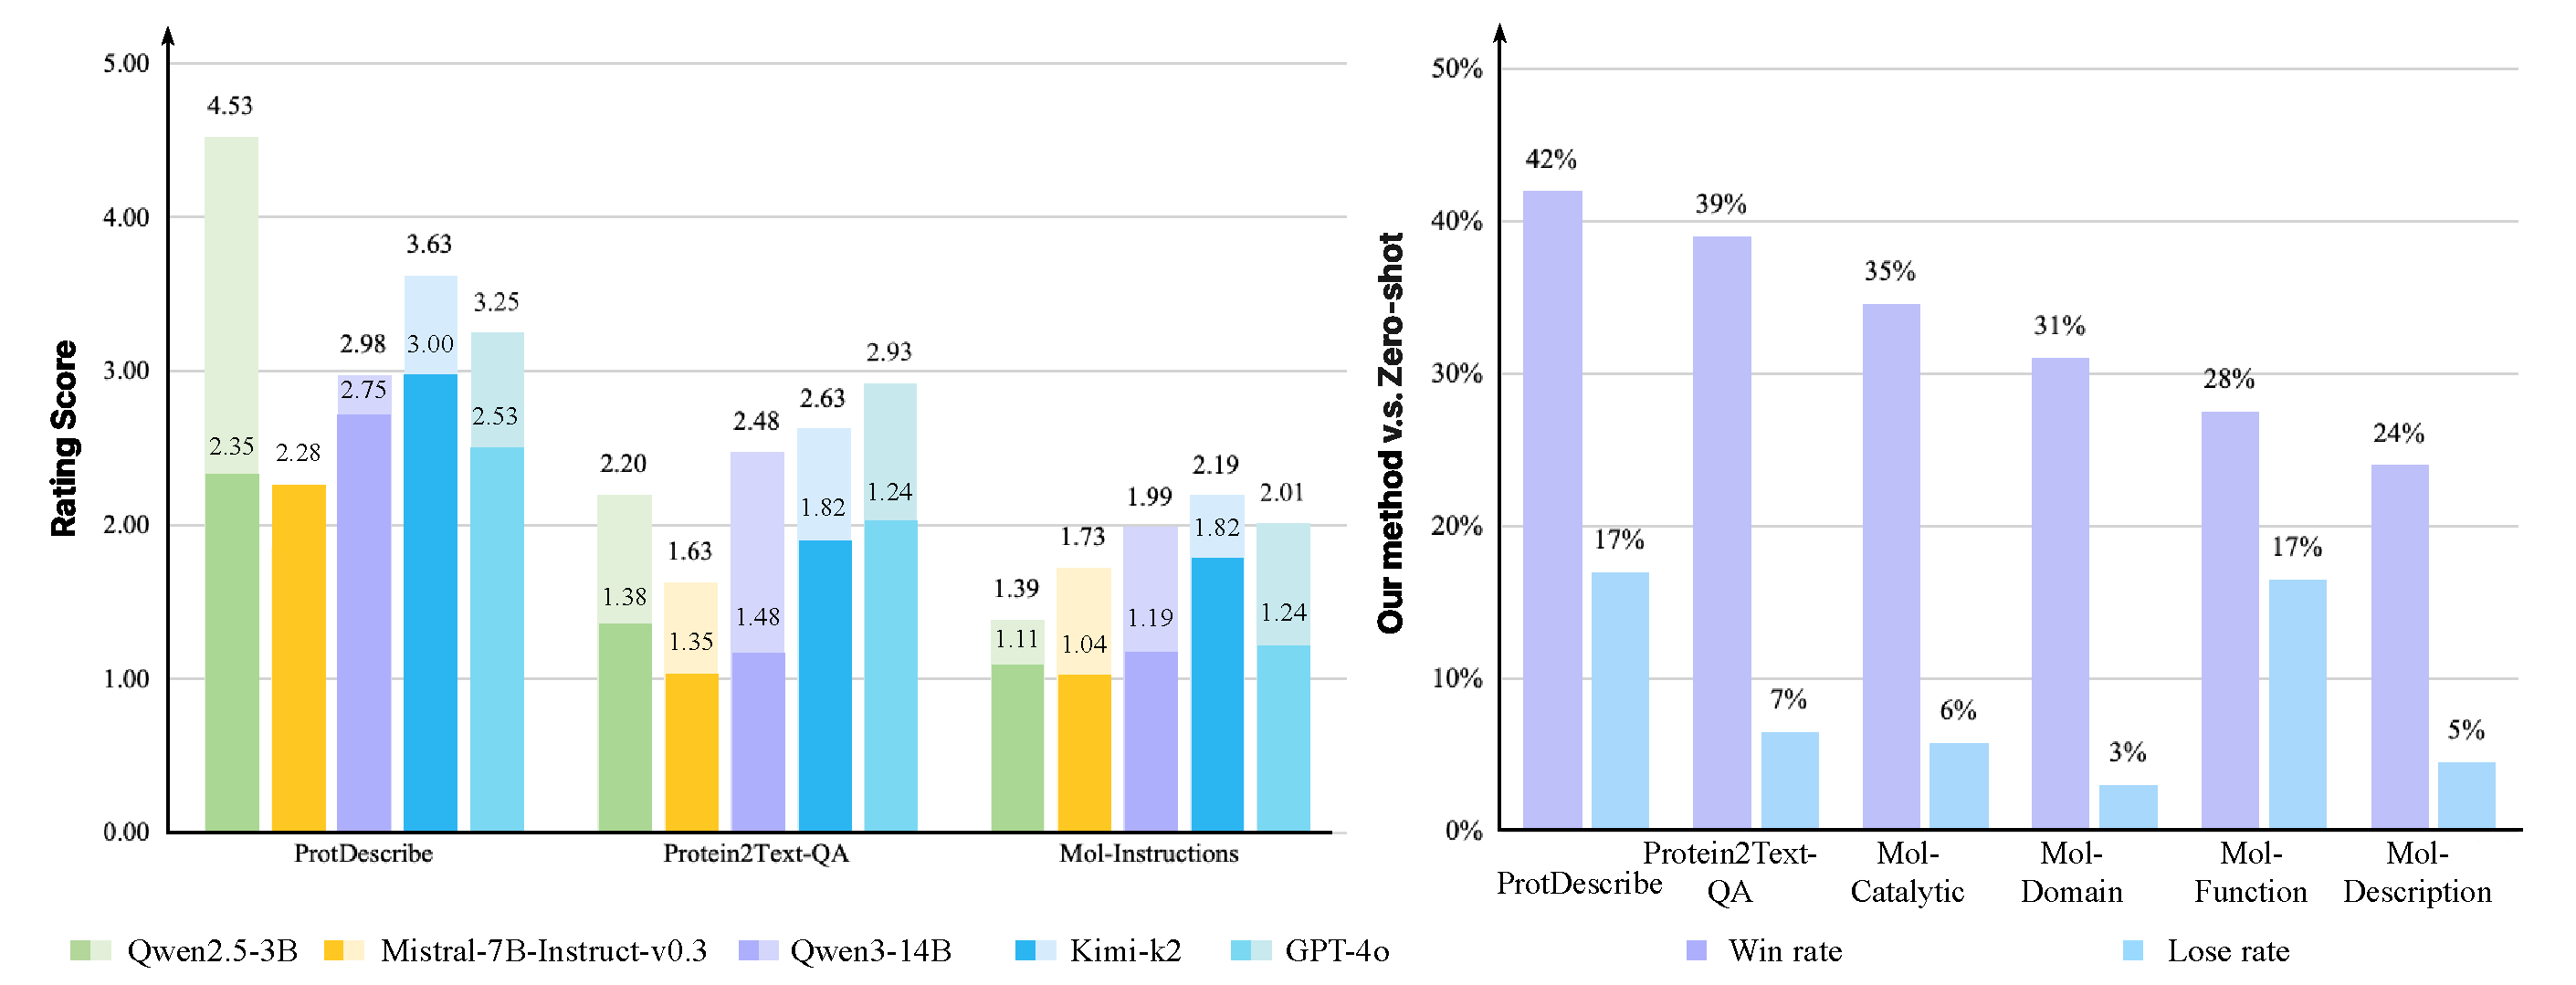
\includegraphics[width=0.9\linewidth]{figure/human_rating_0.pdf}
\caption{\textbf{Comparison of human evaluation results. }
Left: Absolute human rating scores (0–5) for zero-shot model outputs (dark bars) and model outputs with adaptive context exposure (light bars) on three datasets.
Right: Pairwise win/lose proportions comparing outputs with and without adaptive context exposure. Each comparison is based on 8 randomly selected cases per subset (48 cases in total across six subsets).
}
\label{fig:human_rating}
\end{figure}

\paragraph{Varying exemplar number ($k$)}
Figure~\ref{fig:varying_k} illustrates how model performance varies with the number of exemplars ($k$) provided in context across different datasets. Performance generally improves as $k$ increases, but only up to a task-dependent optimum; beyond this point, additional exemplars offer little benefit or even introduce noise. 
% 
The optimal $k$ differs by task. For ProtDescribe~\cite{xu2023protst}, which involves fixed attribute-centric questions, a larger set of bilingual exemplars from related proteins helps the model capture recurring patterns, with performance peaking at $k=10$–$11$. In contrast, Protein2Text-QA~\cite{Protein2Text2025} requires open-ended and integrative reasoning, where only a small number of highly relevant exemplars are beneficial; here, performance peaks earlier at $k=3$–$4$. 
% 
In our experiments, we therefore adopt the task-specific optimal settings: $k=11$ for ProtDescribe~\cite{xu2023protst}, $k=4$ for Protein2Text-QA~\cite{Protein2Text2025}, and $k=4$ for Mol-Instructions~\cite{fang2023mol}. 

\begin{figure}[ht]
\centering
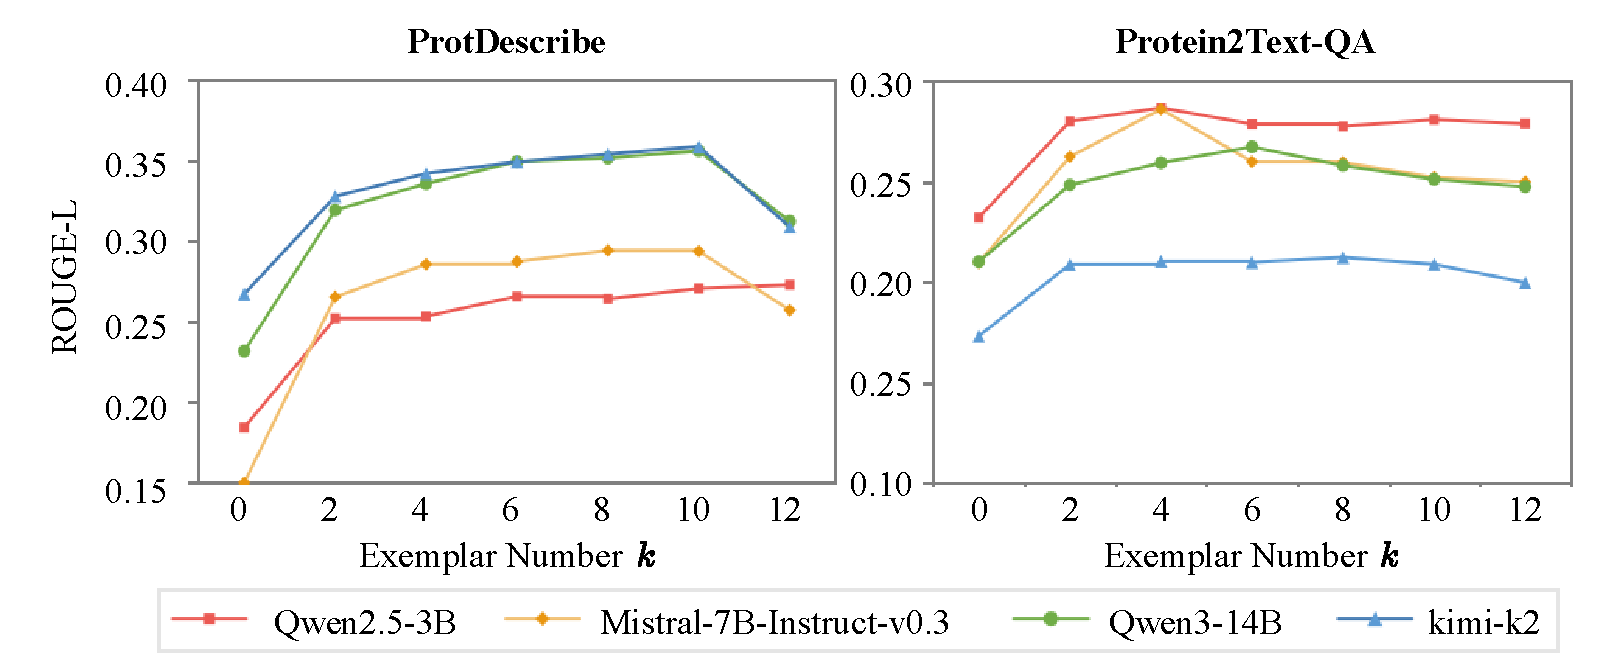
\includegraphics[width=0.72\linewidth]{figure/varying_k_0.pdf}
\caption{\textbf{Effect of varying exemplar number ($k$) on model performance.} We explored $k\in[1,12]$ as the search space; the upper bound was set after a coarse scan up to $k=50$ showed performance saturation around 2-12 exemplars. 
Metric: ROUGE-L.
}
\label{fig:varying_k}
\end{figure}

\paragraph{Ablation on dual-criterion context selection}
Table~\ref{tab:ablation} shows that using both sequence homology and text/QA similarity (Dual) outperforms either criterion alone, providing complementary signals that maximize the effectiveness of context-driven exemplar selection. On average across three datasets, using only sequence homology reduces performance by 5.2\%, and using only text/QA similarity reduces performance by 2.8\% compared to Dual, though all variants still outperform zero-shot models.



\begingroup
\setlength{\tabcolsep}{5
pt}
\begin{table*}[t!]
    \centering
    \caption{\uline{Q3: Each component in \ours positively contributes the performance.}  The original \ours overall performs better than all the variants with some components absent. For each setting, the best performance is highlighted in bold, while the second-best is underlined.
    The mean accuracy values (\%) over five random splits are reported.}
    \label{tab:ablation_study}
\begin{adjustbox}{max width=\textwidth}
\begin{tabular}{c|cccccccccccccccc|c}
\hline
\multirow{2}[2]{*}{\textbf{Dataset}} & \multicolumn{2}{c}{\texttt{coAA}} & \multicolumn{2}{c}{\texttt{coDB}} & \multicolumn{2}{c}{\texttt{coSM}} & \multirow{2}[2]{*}{\texttt{qaBI}} & \multirow{2}[2]{*}{\texttt{qaPH}} & \multirow{2}[2]{*}{\texttt{qaMA}} & \multirow{2}[2]{*}{\texttt{qaST}} & \multirow{2}[2]{*}{\texttt{emEN}} & \multirow{2}[2]{*}{\texttt{emEU}} & \multirow{2}[2]{*}{\texttt{emER}} & \multirow{2}[2]{*}{\texttt{soME}} & \multirow{2}[2]{*}{\texttt{soRE}} & \multirow{2}[2]{*}{\texttt{moML}} & \multirow{2}[2]{*}{Avg.} \bigstrut[t]\\
        & (first) & (last) & (first) & (last) & (first) & (last) &       &       &       &       &       &       &       &       &       &       &  \bigstrut[b]\\
\hline
Stage 1 & 47.53 & 47.65 & 43.42 & 45.84 & 35.75 & 43.38 & 85.52 & 87.15 & 39.24 & 31.20 & 47.14 & 49.08 & 66.01 & 72.83 & 88.94 & 41.88 & 54.54 \bigstrut[t]\\
Stage 2 & 45.83 & 44.27 & 42.67 & 42.71 & 37.14 & 39.83 & 83.85 & 85.41 & 39.32 & 29.18 & 52.21 & 50.73 & 63.32 & 74.27 & \textbf{97.82} & 43.41 & 54.50 \\
No GA & 49.50 & \textbf{50.68} & 45.83 & \uline{49.90} & 40.12 & \uline{48.13} & 86.47 & 87.78 & \textbf{41.03} & 35.96 & 53.07 & \textbf{51.06} & \uline{67.63} & 73.67 & 96.03 & \textbf{44.99} & 57.62 \\
No LF & \uline{49.64} & 50.54 & \textbf{46.63} & 49.86 & \uline{40.53} & \textbf{48.32} & \uline{87.26} & \uline{88.69} & 40.08 & \uline{36.48} & \textbf{54.24} & 50.87 & 66.96 & \textbf{74.91} & \textbf{97.82} & 43.32 & \uline{57.89} \bigstrut[b]\\
\hline
\ours & \textbf{49.68} & \uline{50.60} & \uline{46.55} & \textbf{49.95} & \textbf{40.92} & 48.08 & \textbf{87.41} & \textbf{88.74} & \uline{40.59} & \textbf{36.57} & \uline{53.55} & \uline{50.89} & \textbf{67.77} & \uline{74.87} & \textbf{97.82} & \textbf{44.99} & \textbf{58.06} \bigstrut\\
\hline
\end{tabular}%
\end{adjustbox}
\end{table*}
\endgroup


\paragraph{Case studies and qualitative evaluation}

Figure~\ref{fig:qualitative_examples} illustrates that context-driven exposure produces concise, function-specific descriptions consistent with UniProt annotations. In the two examples shown, the model correctly identifies ``intrinsically disordered regions'', and ``[4Fe-4S] RNA methyltransferase activity'', whereas zero-shot outputs remain generic. 

\begin{figure}[ht]
\centering
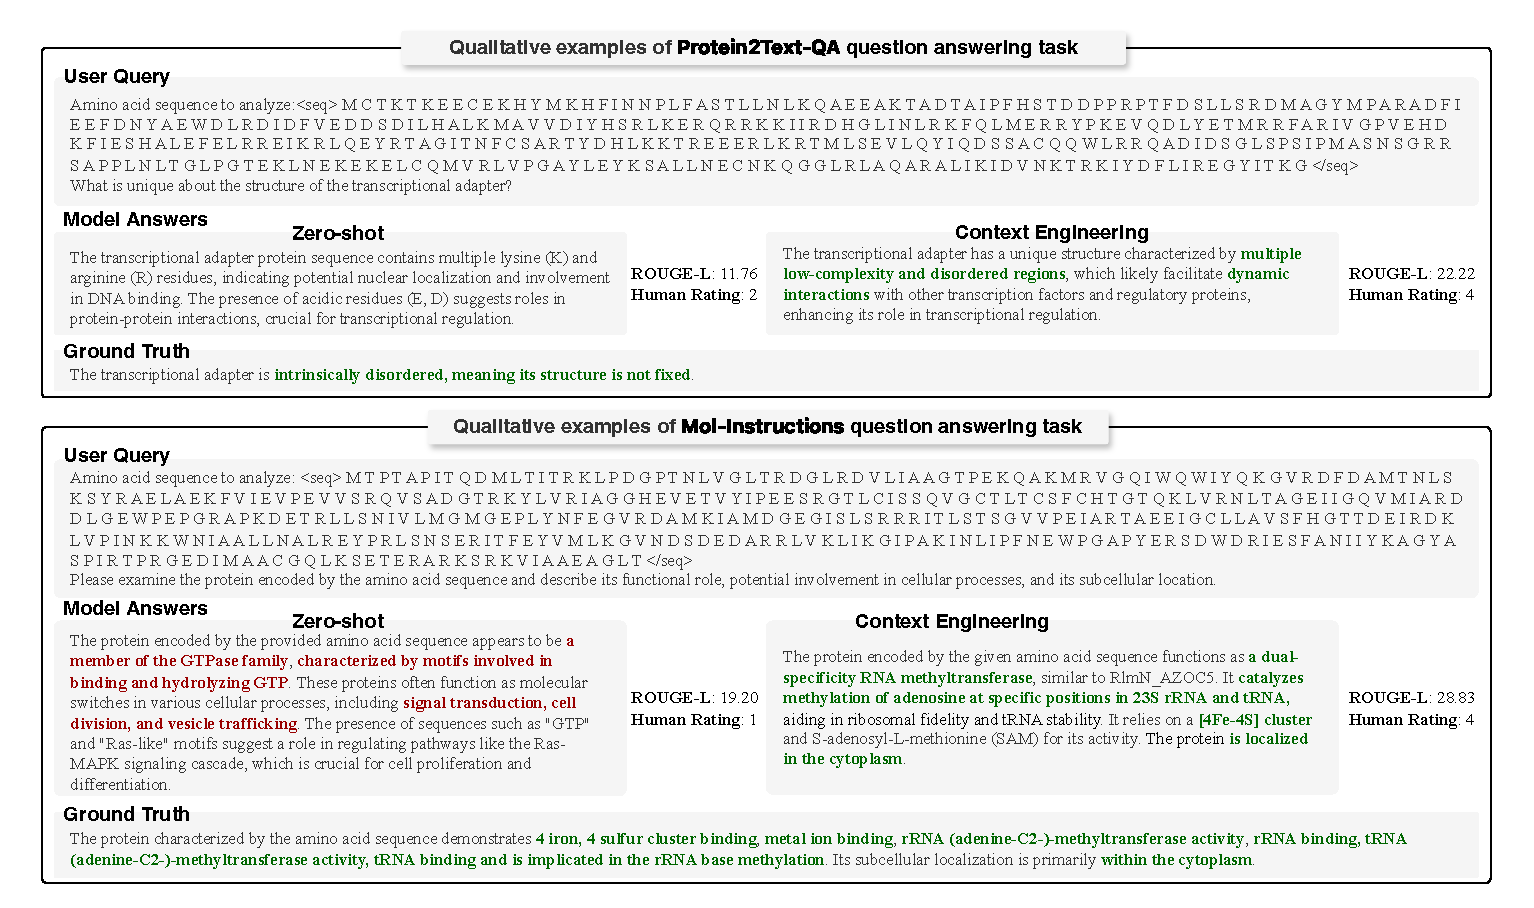
\includegraphics[width=1\linewidth]{figure/qualitative_examples_p2.pdf}
\caption{\textbf{Qualitative examples of protein question answering.} We present two examples with answers generated by GPT-4o~\cite{openai2024gpt4} along with the target ground truth. The green color highlights accurate keywords, while the red color indicates prediction errors.}
\label{fig:qualitative_examples}
\end{figure}